\documentclass[a4paper,11pt]{article}
\usepackage{fullpage}
\usepackage{parskip}

\usepackage{authblk}
\usepackage{apacite}

\usepackage{booktabs}
\usepackage{longtable}
\usepackage{caption}
\usepackage{enumerate}
\usepackage{appendix}

\usepackage{graphicx}
\graphicspath{{images/}}

% Preamble
\title{Time-Space Maps}
\author{Alexandru Cepoi}
\author{Rares Sfirlogea}
\affil{Utrecht University}

% Document
\begin{document}
\maketitle

\section{Introduction}
Understanding the travel time relationships in a transportation system can be crucial
to evaluating its performance. Time--space maps try to show an efficient and easy to
understand portrayal of a transportation network.


\subsection{Definition}
Time space maps are a generalization of the concept of functional spaces where the
physical distance corresponds to the travel time between locations.

Time--space mapping is a method that obtains a spatial configuration of cities (or more
generally points), so that the Euclidean distances between points consist with the given time distances.

\subsection{Terminology}
\begin{description}
    \item[Functional spaces] -- continuous regions generated based on proximity relationships
that generalize the concept of physical distance (these concepts are generally based
on psychological and cognitive distances like transportation flows, social differences
or communication flows)
    \item[Multidimensional scaling (MDS)] -- takes the shortest paths matrix as input and
generates another matrix containing the coordinates of points in time – space
    \item[Distance cartogram] -- map which displays travel times between cities
\end{description}

\subsection{Isochronic Maps}
Are projections of a topographic or other geographical maps displaying accessibility to and/or from a specific central point in travel time. Isochronic maps can also be used to display other types of data like showing accessibility of
number of jobs, potential employees, amenities within a specific time.

\begin{figure}[h!]
  \centering
  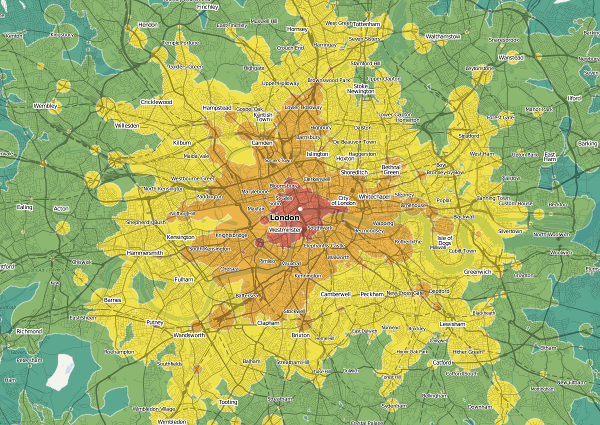
\includegraphics[width=0.8\textwidth]{London.png}
  \caption{Isochronic map of London}
  \label{london}
\end{figure}

\subsection{Tempographic Maps}
These are maps where a transformation of distance to time happens causing a change of
the physical aspect of a country.

\begin{figure}[h!]
  \centering
  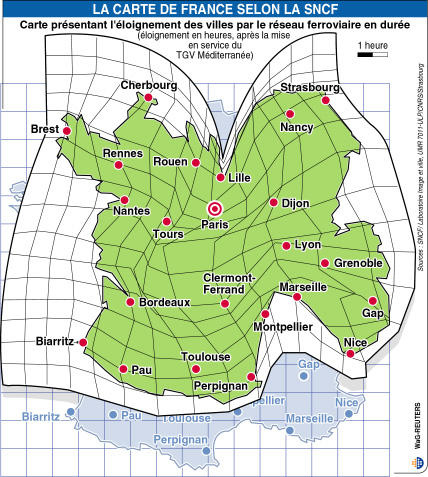
\includegraphics[width=0.5\textwidth]{france.png}
  \caption{Tempographic map of London}
  \label{london}
\end{figure}

\section{Problem Analysis}
\subsection{Literature study \& reverse engineering}
Attempts to generate time-space maps back up to the 1960s. Bunge (1962) portrays two
different time maps for Seattle. The first one uses irregular isochrones (lines of equal travel
time) to show travel times from a specific origin. In the second one the map is distorted in
such manner that the isochrones from the origin become concentric circles.

Ewing and Wolfe (1977) interpolate time--space locations of the transportation network
as well as locations outside the network. After obtaining the set of displacement vectors
they superimpose a uniform grid on the vectors and obtain a warped grid based on the
influence of the vectors. They employ an inverse distance weighting method to interpolate
time–space locations of lattice points of the grid. Marchand (1973) uses for the first time
multidimensional scaling.

In the book Distance and Space, Gaterall (1983) summarizes time--space concepts and
methodologies. He also presents an approach known as Q-analysis (Atkin, 1974, 1981;
Johnson, 1981). This approach focuses on set relations. The set is represented as a graph
based on the connectivity of the nodes of a network to other nodes, degree of incidence and
travel times along the connections. However, this generates an abstract graph that is not
directly comparable with geographic space.

The goal of this study is to analyze and construct a time--space map from a set of travel--time
relations on a specific country.

\subsection{Project Description}
For this study, we are going to focus solely on the Netherlands' railroad transportation
system, there will be no display of travel times to other countries. Judging by the fact that
in this time-space map lakes and other types of landform are irrelevant and may add some
confusion to our end result, only cities, borders and islands will be shown.
The map will have have one central point set at Utrecht and all the cities will be displayed
as a circle with a fixed radius. The travel time will be shown as concentric circles around the
central point set at an $\frac{1}{2}$ hour gap.

\subsection{Issues}
In time–space transformations, the metric nature of time--space is an issue since it is difficult
to represent non-metric spaces as a two-dimensional map or analyze the space using
spatial analytical techniques. The travel times in the origin–destination matrix obtained from
a transportation network may violate one of the metric space axioms, namely, symmetry
(distances between two locations are the same regardless of direction).

The idea of rescaling the physical domain into the temporal domain is old, one of the earliest
examples of time-scaled maps can be found in Tobler(1961) and Bunge (1962) where they
present first examples of small-area scaling. Several works about time scaling follow, most
notable ones are Shimizu (1993) and Spiekerman \& Wegener (1994), in the latter they
construct a two-dimensional time-scaled map of Europe's railroad system using an MDS
algorithm.

Inconclusive results regarding the nature of time--spaces and their structure probably result
from the state of key transformation techniques such as multidimensional scaling (MDS) and
map comparison techniques such as bidimensional regression: these techniques were not
well developed or widely available until recently. Also, previous time--space mapping studies
could not benefit from powerful geographic information system (GIS) software that allow management 
and processing of large and detailed geographic databases as well as tools for
spatial analysis of these data and their product.

\subsection{Statement of the criteria}
Before describing an algorithm for our time--space map it is important to ask ourselves
what accounts for a good time-space map. Strangely this question is not very popular in
the literature and does not have a clear answer. Therefore, we present a set of criteria that
would characterize a good time--space map. By measuring how well our algorithm satisfies
this criteria we have a rough estimation on how well it is performing.

\begin{enumerate}[(i)]
    \item cities must not be placed too close to each other (or overlap)

During the transformation cities can move closer to the central location, others can
move further away. This leads to the possibility that certain cities may need to be placed
very close to one another, which would make the map illegible.

    \begin{center}
        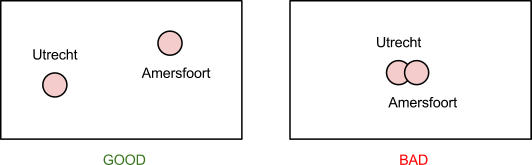
\includegraphics[width=\textwidth]{crit1.png}
    \end{center}

    \item cities must not be placed on water

As cities move on the map to match the time distance, some bad travel connections
could result in pushing a city far from its initial position. It is evidently imposed that whatever
transformation is applied, the city cannot be positioned on water.

    \begin{center}
        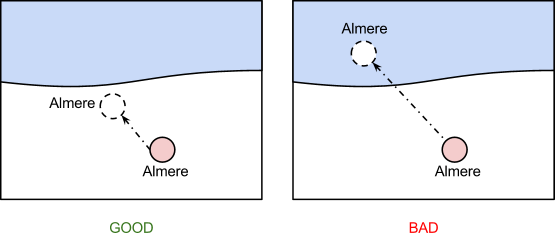
\includegraphics[width=\textwidth]{crit2.png}
    \end{center}
    
    \item cities must not be placed on another island

An obvious problem that can also occur after distortion is modifying the landform
on which the city resides. For this reason, it is mandatory that after the distortion they do
not travel outside their initial land boundaries. For the rest of the paper, when we define an
island as a land areas surrounded by water. Continents are land areas having significant
variation in nature of lands, climate, cultures, etc. For our purposes, when we refer to an island, we may also refer to a continent.

    \begin{center}
        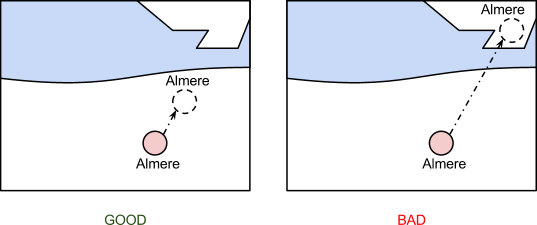
\includegraphics[width=\textwidth]{crit3.png}
    \end{center}

    \item islands must not intersect with other forms of land
    
Another corner case we need to take into account is the possibility of an island to
intersect with another island (or continent for that matter). This is definitely something that
should be avoided, even if it introduces distortion.
    
    \begin{center}
        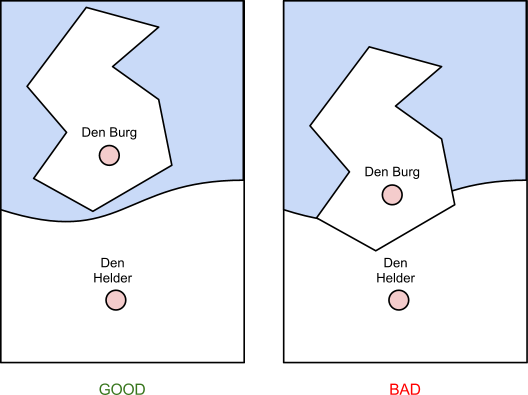
\includegraphics[width=\textwidth]{crit4.png}
    \end{center}
    
    \item keep city orientation
    
The accuracy of the map should not be altered in a way that would affect the reader's
ability to recognize cities by their location on the land forms relative to the selected central
point. Enforcing a limit on the orientation the city will have after distortion will avoid this
situation.
    
    \begin{center}
        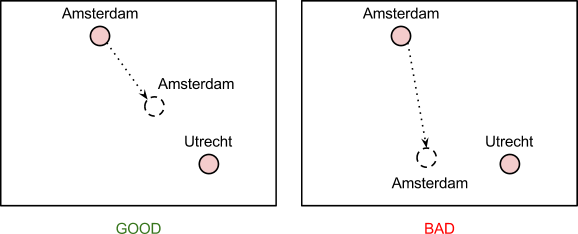
\includegraphics[width=\textwidth]{crit5.png}
    \end{center}
    
    \item cities are not allowed to travel through a bay
    
The most common technique of identifying a city is to memorize its place relative to a
bigger land form. As our time-space map includes only water body elements, the readability
of the map can be further improved by restricting any movement that would traverse a bay.
The actual identification of bays and validity of this criterion will be further explained in
the ``Quantification of the criteria'' section of this paper.
    
    \begin{center}
        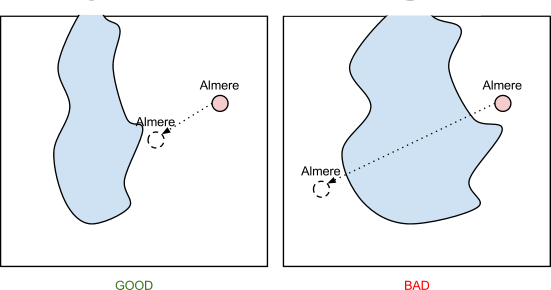
\includegraphics[width=\textwidth]{crit6.png}
    \end{center}
    
    \item border should follow city movement
    
Altering the position of the cities to emphasize the areas where the cities have a
significant better travel connection is not enough to make an easily readable map. Although
it would involve a great distortion of the initial map, moving the border in the direction the
cities are travelling is a mandatory rule that needs to be applied in order to make a good
time-space map. This immediately allows the reader to see the weak spots of the
transportation network.
    
    \begin{center}
        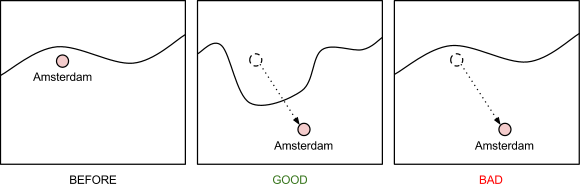
\includegraphics[width=\textwidth]{crit7.png}
    \end{center}

\end{enumerate}

\subsection{Dependency of the criteria}
It is important to analyse the criteria stated above in order to gain a better understanding of
the relationships between them. Some may be very similar, others may depend on another
or there may be conflicting.

Criterion (iii) is very similar to (vi), since both of them constrain cities of travelling through
water. Note that satisfying criterion (vi) also means satisfying (iii). Criterion (ii) is also
similar to these, because it forbids placing a city on water. All these three could be carefully
formulated into a single criteria, but for the sake of clarity and a better quantification, they are
presented distinctly in this paper.

Criterion (i) and (v) impose restrictions on where we can place a city, while (iv) and (vii)
account for border transformations. (iv) and (vii) may come to a conflict because of good
connections to island cities. It is often possible that the border is dramatically altered so that
the island overlaps the continent.

Notice how these three types of criteria all conflict to some extent with each other, since
imposing some very strict restrictions on one of them leads to higher degrees of distortion
in the others. For example, imposing criterion (i) may render satisfying (v) completely
impossible, since two cities may want to overlap, and we need to respect the time scale. We
have found that for every one of these criteria there is a corner case in which achieving a
smaller distortion in one would render a higher distortion at least one of the others. A good
solution would need to find the best trade-offs in satisfying all of them.

\subsection{Quantification of the criteria}

Now that we have determined our criteria, we can describe proper formal requirements. In
general we will have two types of criteria, binary constraints, implying that some condition
that the output of our algorithm must satisfy, and in quantitative manner, for which we
would define a general quality function. This approach suggests the intent of minimizing
or maximizing a specific value for a better quality output. A distortion function usually
involves minimizing a value, while a quality function must be maximized. Since defining a
distortion function $f$ is analogous to defining a quality function as $1/f$, we will use the two
interchangeably.

\begin{enumerate}[(i)]
    \item cities must not be placed too close to each other (or
      overlap)

      In order to properly define ``closeness'' in this context, it is
      important to realize that this criterion depends strictly on the
      scale of the map we are rendering, since its main role is purely
      esthetic (readability).

      A reasonable quantification would be to enforce the distance
      between two cities to be at least two times the city point
      diameter. This would be what we call a hard or binary
      constraint.

    \begin{center}
        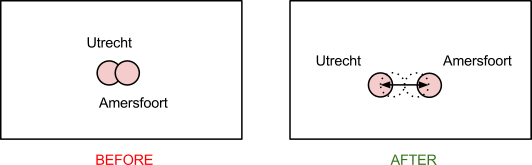
\includegraphics[width=\textwidth]{quant1.png}
    \end{center}
    
    \item cities must not be placed on water

      This is another simple binary constraint. When moving a city to
      match the time travel times, it should never end up in the sea
      or ocean. A more general approach to this issue is that the land
      in its immediate vicinity should move along with it.

    \item cities must not be placed on another island

      Very similar with the criterion above, this enforces that a city
      must end up on the same island after the
      transformation. However, the “same island after the
      transformation” construct deserves a more formal
      explanation. While we can easily formalize “same island” as the
      existence of a land path between two points, the implication of
      the transformation itself makes this definition vague.

      Assuming we are to place 4 anchors evenly distributed around a
      city point, they will always end on the land or on the
      coastline. Complying to this criterion would mean checking that
      after the transformation there is a continuous land path between
      the city center and all of the 4 control points.

    \item islands must not intersect with other forms of land

      This binary criterion states that none of the islands after the
      transformation are allowed to overlap. A basic requirement for
      most map transformations.
    
    \item keep city orientation
      
      The map transformation should change the distances between the
      central point and different cities, but not the angle between
      them. We define the angle of two cities as the angle made by the
      straight line which joins them and the West-East axis. Due to
      the imposed restrictions (for example due to the fact that
      cities are not allowed to overlap), we cannot guarantee that
      this angle would always be the same. Therefore we need to
      describe a quantitative way of measuring the distortion
      introduced.

      A first naive approach would be to define the distortion as the
      difference in the angles from before and after the
      transformation, but as we can see in the figure below. this is
      not a very good one, since $30^{\circ}$ angle of distortion
      accounts for moving a city 10 or 20 km depending on how far it
      is. If we were to create a time scaled map of Europe, moving
      Amersfoort (a town very close to Utrecht) a few kilometers south
      would produce the same distortion as placing Warsaw next to
      Milan for example.

      A better approach would be to measure the distortion in
      kilometers or miles. However 20 kilometers' worth of distortion
      would give $45^{\circ}$ of freedom for placing Amersfoort and $2-3^{\circ}$ of
      freedom for Groningen.

      The best approach would be to define inversely proportional
      relationship between the angle and distance. If we note the
      angle measured in degrees($^{\circ}$) with a and distance
      measured in km with $d$, the most simple example would be the
      product $da$. Variants such as $d\log{a}$ could be used to
      decrease the importance of the angle in the product. The
      convolution $d*a$ is another option which probably deserves more
      investigation. For our purposes we found that the product d a
      works well enough so we will use that to measure the distortion
      introduced by variations in the original angle. A table with
      possible variation of the same distortion error is presented
      below.

      \begin{center}
      \begin{tabular}{llllll}
        \toprule
        distance$(d)$ & 10km & 30km & 50km & 100km & 150km\\
        \midrule
        angle$(a)$ & $90^{\circ}$ & $30^{\circ}$ & $18^{\circ}$ &
        $9^{\circ}$ & $6^{\circ}$\\
        \bottomrule
      \end{tabular}
    \end{center}
      
    \begin{center}
        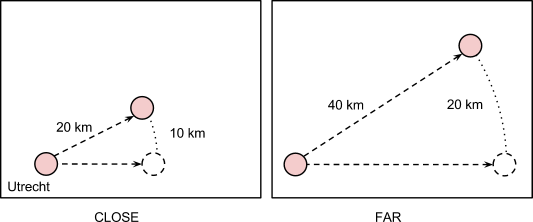
\includegraphics[width=\textwidth]{quant5.png}
    \end{center}
    
    \item cities are not allowed to travel through a bay

      Before we formalize this criterion we need to define a bay. A bay
      is a large body of water formed by an inlet of land. $A$ bay can
      be a gulf, an inner sea, a lake, etc. Let us assume we want to
      move a city from $A$ to $B$ during a transformation algorithm (see
      figure below). We name as control segments all the intersections
      of segment $[AB]$ with water before and after applying the
      algorithm. Notice that $A$ and $B$ are on land (or on the coastline)
      so at the very least the union of all control segments before
      the transformation is included in $(AB)$. Same thing applies to
      all control segments from the map generated by the
      transformation.

      We define mapping $A$ to $B$ as ``acceptable'' with respect to $d$
      (where $d$ is a real number) if and only if for all control
      segments $C_iC_j$ we have a land path from $C_i$ to $C_j$ within the area
      defined by the circle with diameter $d$ and center in the midpoint
      $[C_iC_j]$.  The land path here is respective to the map the control
      segment belongs to (either the original map or the transformed
      map).

      We say that the transformation of the map is ``acceptable'' with
      respect to d if all of its mappings are ``acceptable'' with
      respect to $d$. We can now introduce a distortion function to
      this criterion as the minimum real number $d$ (measured in km)
      with respect to which the transformation is acceptable. Our
      algorithm should seek to minimize this number.

    \begin{center}
        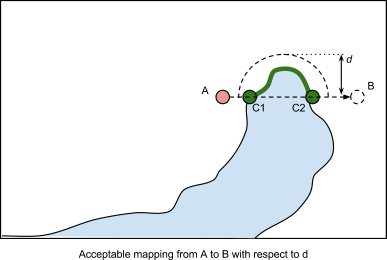
\includegraphics[width=0.6\textwidth]{quant6.png}
    \end{center}
    
    \item border should follow city movement
      
      It should be clear by now that the border should be deformed to
      accommodate for changes in the surroundings. It is not realistic
      that all the cities nearby are pulled towards the center
      (assuming they have really good connections) but the coast
      remains far apart. It is even unrealistic to assume the speed
      with which we can travel towards the border is the same as the
      speed with which we travel towards the cities on the way
      there. Generally speaking there are so many unknowns in this
      equation that it is questionable whether we should even define a
      distortion function for this criterion. Still this is one of the
      most problematic aspects of the project and having some (even
      highly) rough estimations on how an algorithm is fairing is
      crucial to assess and improve it.

      We start by selecting a point $X$ on the border and assume our
      algorithm has generated a time $t$ to get from the center($U$) to
      $X$. We will define a distortion function $d(a)$ which returns a
      distortion based on an angle parameter a. First of all, we
      select an angle of $d(a)$ such that $UX$ is its bisection (see
      figure below) and gather all the cities which are not farther
      away (in distance) than $X$.

      For each of the cities mentioned, we calculate the total time it
      would take to reach $X$ through that city, assuming constant
      speed. For example estimated time for getting to X through A
      would be $t(UA)(1 + \frac{d(AX)}{d(UA)})$.

      For this time we set a weight of $\frac{1}{d(AX)}$ and then calculate the
      weighted average for all the cities within the aforementioned
      angle. This step ensures preference for the closest cities,
      favoring a decent connection to a close city ($B$ for example)
      over an excellent one to a farther city (in this case $A$).

      Finally we set $d(a)$ as the absolute value of the difference
      between the reported time $t$ and the calculated weighted
      average. Although arguably an algorithm in its own right (albeit
      simple and naive) this distortion function keeps the main
      algorithm in check (at least to some extent) with one of the
      most basic approaches of solving this problem.

    \begin{center}
        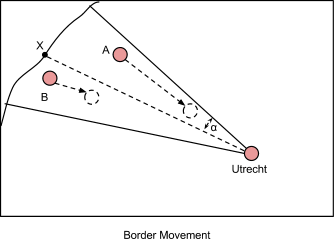
\includegraphics[width=0.6\textwidth]{quant7.png}
    \end{center}
\end{enumerate}

\section{Algorithm design}

\subsection{Specification of the input and output}

Building a map that outlines the transportation system of a country involves knowing some initial variables. As our focus was directed towards building a time space map of the Netherlands we will receive as input the following data:

\begin{enumerate}[(i)]
	\item Map of the Netherlands
	
		This will be represented as a list of cyclic points which build into polygons. A polygon is closed (we have an island) when the next point read is equal to the first one. The list may contain multiple islands.
		
		\emph{Example:} (28,19), (81,7), (137,20), (173,49), (129,111), (94,71), (62,82), (65,124), (11,124), (28,19), (202,37), (200,57), (225,62), (223,21), (202,37)

	\item List of cities
	
		The list will be encoded as a JSON array with each element representing a city. Each component of the array will include the following details: name, position, best travel time to central city.
\end{enumerate}

\subsection{Algorithmic problem statement}

The problem is solved.

\subsection{Algorithm development}

\begin{figure}[h!]
  \centering
  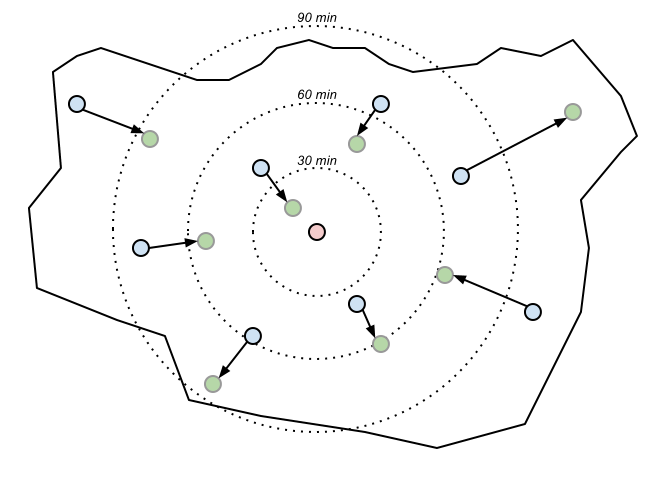
\includegraphics[width=0.8\textwidth]{forces.png}
  \caption{City movement vectors}
  \label{forces}
\end{figure}

\begin{figure}[h!]
  \centering
  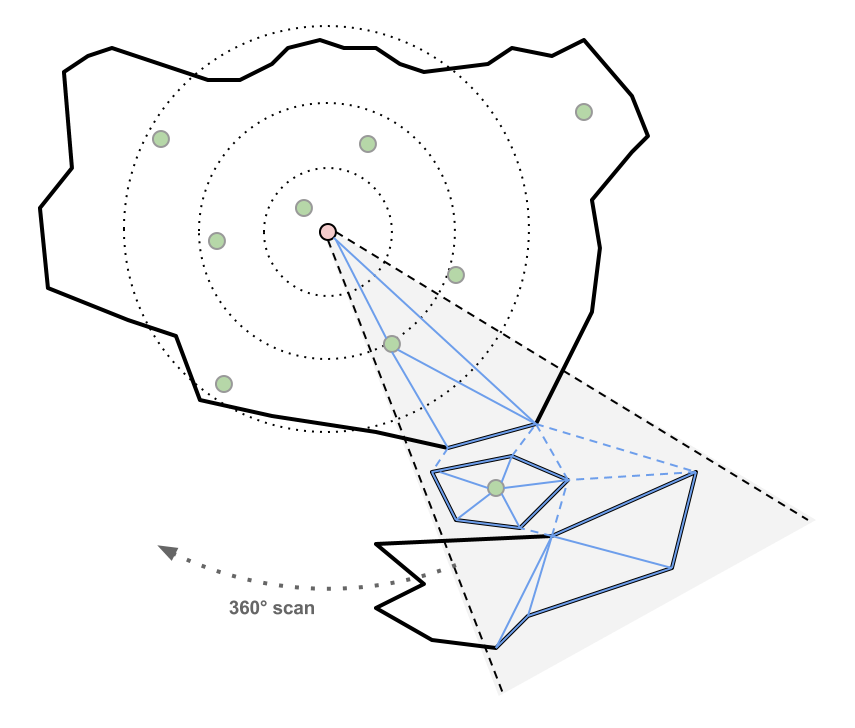
\includegraphics[width=0.8\textwidth]{scan.png}
  \caption{Ray scanning for triangulation}
  \label{scan}
\end{figure}

\subsection{Efficiency analysis}
Triangulation can be achieved in linear time \cite{chazelle}.

% references
\bibliographystyle{apacite}
\bibliography{references}

\end{document}